%!TEX TS-program = xelatex 
%!TEX TS-options = -output-driver="xdvipdfmx -q -E"
%!TEX encoding = UTF-8 Unicode
%
%  ethics_syllabus
%
%  Created by Mark Eli Kalderon on 2007-10-01.
%

\documentclass[12pt]{article} 

% Definitions
\def\mykeywords{ethics, syllabus, Hume, Kant, Nietzsche} 
\def\myauthor{Mark Eli Kalderon} 
\def\mytitle{Introduction to Moral Philosophy}
\def\svncommitter{kalderon}

% Packages
\usepackage{geometry} \geometry{a4paper} 
\usepackage{url}
\usepackage{pdfsync} 
\usepackage{txfonts}
\usepackage{color}
\definecolor{gray}{rgb}{0.459,0.438,0.471}
\usepackage{setspace}
% \doublespace % Uncomment for doublespacing if necessary
% \usepackage{epigraph} % optional

% XeTeX
\usepackage[cm-default]{fontspec}
\usepackage{xltxtra,xunicode}
\defaultfontfeatures{Scale=MatchLowercase,Mapping=tex-text}
\setmainfont{Hoefler Text}
\setsansfont{Gill Sans}
\setmonofont{Inconsolata}

% Version Control Information
\usepackage{svn-multi}
\svnidlong
{$HeadURL$}
{$LastChangedDate$}
{$LastChangedRevision$}
{$LastChangedBy$}
\svnRegisterAuthor{\svncommitter}{Mark Eli Kalderon}
% Make sure to run the following to set the svn keywords:
% svn propset svn:keywords 'HeadURL LastChangedDate LastChangedRevision LastChangedBy' /Users/markkalderon/Documents/TheHub/Teaching/Intro_Ethics/README.txt


% Section Formatting
\usepackage[]{titlesec}
\titleformat{\section}[hang]{\fontsize{14}{14}\scshape}{\S{\thesection}}{.5em}{}{}
\titleformat{\subsection}[hang]{\fontsize{12}{12}\scshape}{\S{\thesubsection}}{.5em}{}{}
\titleformat{\subsubsection}[hang]{\fontsize{12}{12}\scshape}{\S{\thesubsubsection}}{.5em}{}{}

% Headers and Footers
% \usepackage{fancyhdr}
% \pagestyle{fancy}
% \pagenumbering{arabic}
% \lhead{\thepage}
% \chead{}
% \rhead{\itshape{\nouppercase{\leftmark}}}
% \lfoot{\tiny{URL: \url{\svnkw{HeadURL}} ; \space Last changed on: \svndate ; \space Revision: \svnrev ; \space Author: \svnFullAuthor*{\svnauthor}}}
% \cfoot{}
% \rfoot{}

% Bibliography
% \usepackage[round]{natbib} 

% Title Information
\title{\mytitle}% Thanks optional 
\author{\myauthor} 
\date{} % Leave blank for no date, comment out for most recent date

% PDF Stuff
\usepackage[plainpages=false, pdfpagelabels, bookmarksnumbered, backref, pdftitle={\mytitle}, pagebackref, pdfauthor={\myauthor}, pdfkeywords={\mykeywords}, xetex, colorlinks=true, citecolor=gray, linkcolor=gray, urlcolor=gray]{hyperref}

%%% BEGIN DOCUMENT
\begin{document}

% Title Page
\maketitle
% \begin{abstract} % optional
% \end{abstract} 
% \vskip 2em \hrule height 0.4pt \vskip 2em
% \epigraph{text of epigraph}{\textsc{author of epigraph}} % optional; make sure to uncomment \usepackage{epigraph}

% Layout Settings
\setlength{\parindent}{1em}

% Main Content

\begin{figure}[htbp]
    \centering
        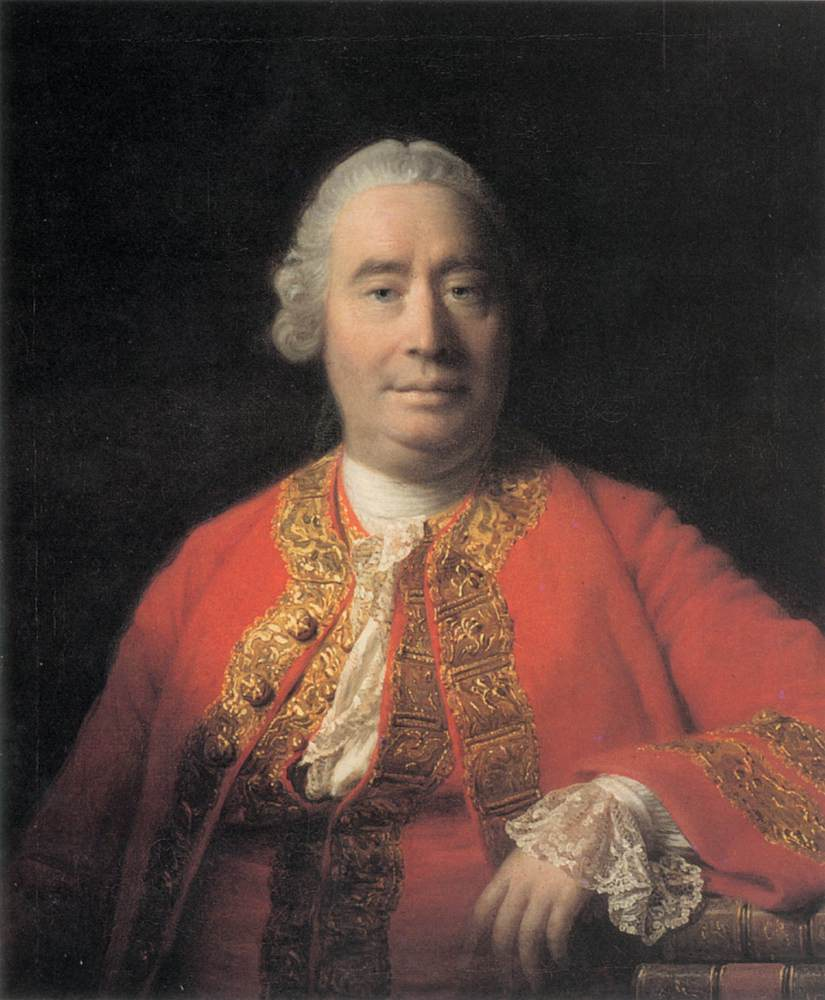
\includegraphics[height=4cm]{../Hume/Graphics/hume.jpg}
        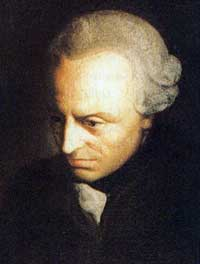
\includegraphics[height=4cm]{../Kant/Graphics/kant.jpg}
        \includegraphics[height=4cm]{../Nietzsche/Graphics/N.jpg}
    % \caption{caption}
    \label{fig:Pictures_kant}
\end{figure}

\section{Description}\label{sec:description} % (fold)

The aim of these lectures is to introduce the student to the central themes of moral philosophy through the close examination of key historical texts. The objective is to provide the student with an in depth undersanding of these texts and to provide the student sufficient background for further study of both the texts under study and moral philosophy more generally.

% section description (end)

\section{Reading}\label{sec:reading} % (fold)

The primary historical texts that we will be studying are:
\begin{itemize}
    \item David Hume, \emph{A Treatise of Human Nature}, Book III, David Fate Norton and Mary J. Norton (eds.), Oxford: Oxford University Press, 2003.
    \item Immanuel Kant, \emph{Groundwork for the Metaphysics of Morals}, Mary Gregor (ed.), Cambridge: Cambridge University Press, 2002.
    \item Friederich Nietzsche, \emph{On the Genealogy of Morals}, Walter Kaufman (ed.), New York: Vintage Books, 1990.
\end{itemize}

The secondary literature on these topics is vast and difficult. For now, students should spend their time and energy trying to understand Hume, Kant, and Nietzsche rather than trying to understand their commentators. However, if some extra guidance is needed, I would recommend the following two books:
\begin{itemize}
    \item John Rawls, \emph{Lectures on the History of Moral Philosophy}, Cambridge, MA: Harvard University Presss, 2000.
    \item David Wiggins, \emph{Ethics: Twelve Lectures on the Philosophy of Morality}, London: Penguin Books, 2006.
\end{itemize}

% section reading (end)

\section{Online Resources}\label{sec:online_resources} % (fold)

Lecture notes will be posted online. These are available at:
\begin{quote}
	\url{http://markelikalderon.com/teaching/}
\end{quote}
These are updated semi-regularly. It is best to download these \emph{after} the lecture as the material can change to reflect the current lectures. Also, the online versions will contain some material not presented in lecture.

% section online_resources (end)

\section{Backup Classes}\label{sec:backup_classes} % (fold)

Backup classes are available to non-philosopy students attending these lectures as a course unit. The backup classes are taught by Nadine Elzein and are in Room G17, Pearson Building (North East Entrance), Thursday 1--2.

% section backup_classes (end)

\section{Contact Information}\label{sec:contact_information} % (fold)

Mark Eli Kalderon\\
Room \textsc{b}02, 19 Gordon Square\\
(0)20 7679-3577\\
Office Hours: 2--3\textsc{pm} Thursday\\
\href{mailto:m.kalderon@ucl.ac.uk}{m.kalderon@ucl.ac.uk}\\
\url{http://markelikalderon.com}

% section contact_information (end)


% Bibligography
% \bibliographystyle{plainnat} 
% \bibliography{Philosophy.bib} 

\end{document}
